% A good introduction to latex can be found here:
%    http://www.cse.ohio-state.edu/~hank/latex/lshort141.pdf

\documentclass[9.5pt]{extarticle}

\usepackage{full page}  % make the margins somewhat smaller than the default
\usepackage{graphicx}
\usepackage{amsmath}
\usepackage{indentfirst}
\usepackage{color}
\usepackage{cite}
\usepackage{wasysym}
\usepackage{amssymb}
\usepackage{multirow}
\usepackage{float}
\usepackage{lscape}
\usepackage{alltt} 
\usepackage{listings}
\usepackage{booktabs}
\usepackage{mathtools}
\usepackage{fancyhdr}
\usepackage[table,xcdraw]{xcolor}

\DeclarePairedDelimiter{\ceil}{\lceil}{\rceil}
\DeclarePairedDelimiter{\floor}{\lfloor}{\rfloor}

\definecolor{dkgreen}{rgb}{0,0.6,0}
\definecolor{gray}{rgb}{0.5,0.5,0.5}
\definecolor{mauve}{rgb}{0.58,0,0.82}


\usepackage{listings}  %  needed for source code listings

\lstset{frame=tb,
  language= java,
  aboveskip=1.5mm,
  belowskip=1.5mm,
  showstringspaces=false,
  columns=flexible,
  basicstyle={\small\ttfamily},
  keywordstyle=\color{blue},
  commentstyle=\color{dkgreen},
  stringstyle=\color{mauve},
  breaklines=true,
  tabsize=2,
  numbers=left,
  stepnumber=1,    
  firstnumber=1,
  numberfirstline=true
}
       

% set the document title, author, and date here.
%  once set, the \maketitle command (within the document)
%  will display them nicely
\title{Motion Planning Assignment}
\author{Chua Zheng Fu Edrei}

\begin{document}
\maketitle

\section{Introduction}

In this report, we present motion planning algorithm using Probabilistic Roadmap (PRM) and Rapidly Exploring Random Tree (RRT). We also discuss the results and attempt to perform optimization.

\section{Probabilistic Roadmap}

\subsection{Implementation}

The basic idea behind PRM is to plant random nodes from the configuration space of the robot, test if there are in a collision-free space and make use of a planner (PRMPlanner) to connect each collision-free configuration to nearby configuration. A* search is used to find a path between the start and the goal configurations. \\

A graph, \verb`Map<Vector, Map<Vector, Double>> roadMap` is used as the data structure for PRM. There are 3 important functions that are implemented in PRMPlanner.java: \verb`generateFreeConfiguration`, \verb`growMap`, \verb`addVertex` and the code is given in Listing 1 - 3.\\

\verb`generateFreeConfiguration` returns a valid configuration randomly if one is found in \verb`numberOfAttempts` time.  \verb`growMap` attempts to add $K$ collision free configuration to the roadmap. Finally, \verb`addVertex` add the new configuration to the roadmap and insert an edge between the vertex and its $k$ nearest neighbour if there exists a collision free trajectory.\\

\begin{lstlisting}[language=java,caption={Java code for addVertex}]
List<Vector> neighbours = nearestKNeighbors(roadMap.keySet(),free,kValue());
roadMap.put(free, new HashMap<>());
for(Vector v: neighbours) {
	if (getEnvironment().isSteerable(getRobot(), free, v, RESOLUTION) &&
		getEnvironment().isSteerable(getRobot(), v, free, RESOLUTION)) {
		roadMap.get(free).put(v, getRobot().getMetric(free, v));
		roadMap.get(v).put(free, getRobot().getMetric(free, v));
	}
}
\end{lstlisting}

\begin{lstlisting}[language=java,caption={Java code for generateFreeConfiguration}]
for(int i=0; i<numberOfAttempts; i++){
	Vector config = getRobot().getRandomConfiguration(getEnvironment(),random);
	if(getEnvironment().isValidConfiguration(getRobot(), config)) return config;
}
return null;
\end{lstlisting}

\begin{lstlisting}[language=java,caption={Java code for growMap}]
for (int i = 0; i < K; i++) {
	Vector config = generateFreeConfiguration();
	addVertex(config);
}
\end{lstlisting}

\subsection{Testing}

To test the PRM algorithm, we used a robot arm configuration (robot\_arm\_environment) and planted 1000 nodes. The movement of the robot arm is given in Figure 1. On my machine (MacBook i5 2.5G dual core), growing1000 nodes takes 55 seconds and a path is found with error 0. More elaborate testing and optimization will be discussed in subsequent section.

\begin{figure}[H]
\centering
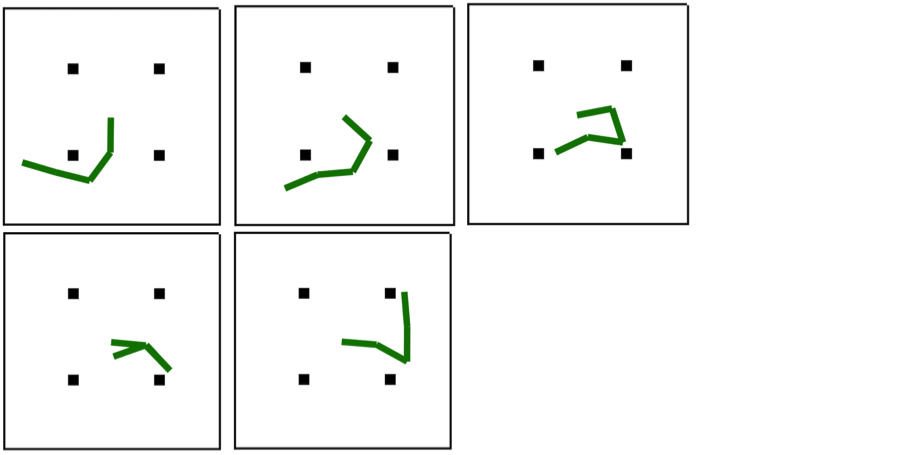
\includegraphics[scale=1]{prm1.png}
\caption{PRMPlanner on robot\_arm\_environment with MotionPlanner.RESOLUTION = 0.01, MotionPlanner.defaultSize = 1000, PRMPlanner.numberOfAttempts = 10, kValue = 15, and default start/goal }
\label{Figure 1}
\end{figure}


\section{Rapidly Exploring Random Tree}

\subsection{Implementation}

The basic idea of a Rapidly Exploring Random Tree (RRT) is to grow a tree rooted at the starting configuration with random nodes branching out. A connection is established between a node and its nearest neighbour if it is collision-free. Because the sampling is random, the tree expands towards large unsearched area. In the query phase, we find the node that is nearest to the goal and perform backtracing on the tree to the start state.\\

The tree data structure is represented by \verb`Map<Vector, Edge> parents`. \verb`Edge` stores the configuration of the parents (to allow for backtracking), the control and duration (to obtain the trajectory) and a pair of points (to allow for plotting for edges) and the data structure is implemented as a class in RRTPlanner.java.\\

There are three important functions in RRTPlanner.java: \verb`growMap`, \verb`newConf` and \verb`findPath` and they are given in Listing 4 to 6.\\

\verb`growMap` attempts to add $K$ collision-free configuration to the tree and does it by generating a random configuration and finding its nearest neighbour, and the process is iterated $K$ times. \verb`newConf` adds a new configuration to the graph by applying a random control at \textit{qnear} for \textit{duration} units of time and adding an edge if the trajectory is collision free. Finally, \verb`findPath` performs the backtracing from the goal state to the start state by accessing the parent configuration stored in the \verb`Edge` class.\\

\begin{lstlisting}[language=java,caption={Java code for growMap}]
while( i < K ){
	Vector qrand = getRobot().getRandomConfiguration(getEnvironment(), random);
	Vector qnear = nearestNeighbor(parents.keySet(), qrand);
	if(newConf(qnear, DEFAULT_DELTA)) i++;
}
\end{lstlisting}

\begin{lstlisting}[language=java,caption={Java code for newConf}]
Vector control = getRobot().getRandomControl(random);
Vector end = getRobot().move(qnear,control,duration);
if(getEnvironment().isValidMotion(getRobot(),qnear,new Trajectory(control,duration),RESOLUTION)) {
	if(!parents.containsKey(end)){
		parents.put(end, new Edge(qnear, control, duration));
		return true;
	}
}
return false;
\end{lstlisting}

\begin{lstlisting}[language=java,caption={Java code for findPath}]
Vector goal = nearestNeighbor(parents.keySet(),getGoal());
Trajectory result = new Trajectory();
Vector node = goal;
while(true){
	Edge e = parents.get(node);
	Trajectory temp = new Trajectory(e.getControl(),e.getDuration());
	temp.append(result);
	result = temp;
	node = e.getConfiguration();
	if(node.equals(getStart()))
		return result;
}
\end{lstlisting}

\subsection{Testing}

To test the RRT algorithm, we used a differential drive robot in the planar\_robot\_environment. On my machine (MacBook i5 2.5G dual core), growing 20000 nodes takes 158 seconds with a path error 0.4. More elaborate testing and optimization will be discussed in subsequent section.

\begin{figure}[H]
\centering
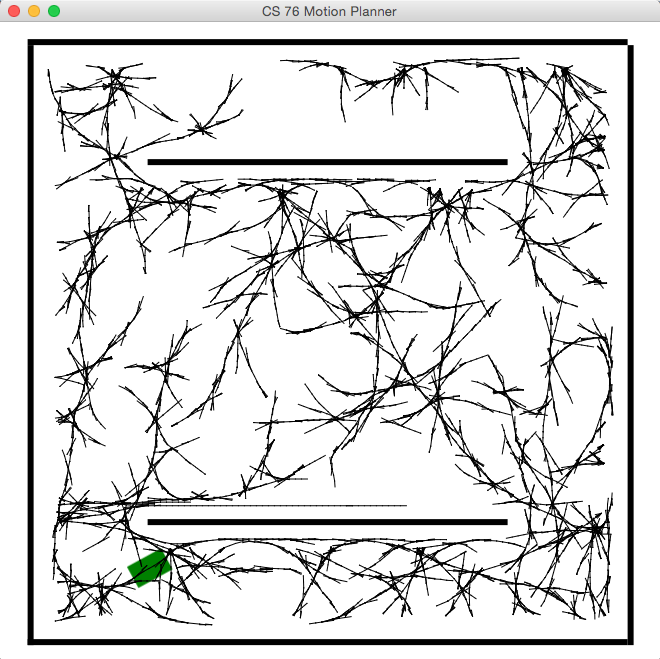
\includegraphics[scale=0.4]{rrt1.png}
\caption{RRTPlanner on planar\_robot\_environment with differential drive robot, MotionPlanner.RESOLUTION = 0.01, MotionPlanner.defaultSize = 20000, and default start/goal}
\label{Figure 2}
\end{figure}

\section{Questions and Experiments}

Even if a feasible trajectory exists, PRM and RRT is not guaranteed to find a feasible trajectory within a finite time. This is because PRM and RRT is essentially a random (or Monte Carlo) algorithm and randomness might not always work in the way we expect in a finite time. Suppose the \verb`getRandomConfiguration` function of PRM and RRT decides by randomness to only explore the space near the start and there are no nodes near the goal. In this case, the algorithm might not be able to plot a trajectory to the goal. Monte Carlos algorithm simply assume the law of large number works, which is generally the case, but is not guaranteed.\\

PRM has the advantage that it is fast. In addition, it can be used to support multi-query. Once the roadmap is built, the program can query multiple times to plan a path connecting any two nodes. However, PRM works only when the environment is static (or does not change much). RRT has the advantage that it can deal with dynamic environment since the sampling is conducted during the search process. However, it has to be performed again each time we change the  goal configuration and is suited for single-query. Therefore, I will use PRM if I know that I need to plan for multiple start and goal configuration in a relatively static environment, and I will use RRT if I know that the start state  is going to be fixed (single query) or the environment is dynamic.\\
  
Based on the result from profiling using VisualVM and the benchmark program, I noted that the bottleneck for PRM planner is in the collision detection phase. In order to optimize the PRM search, I performed ``lazy PRM''. Further discussion of the implementation and experiment is in the optimization section.\\

Based on the test run, I noted that the path quality for the RRT planner is bad (there is a lot of unnecessary adjustment of the robot). I implemented serveral optimizations (randomized delta value, goal bias and path shortening) and discussion of the implementation and experiment is in the optimization section.\\

\section{Optimization}
\subsection{PRM Planner}

To run the optimized algorithm, set the \verb`optimize` variable in the header of PRMPlanner.java to \verb`true`.

\subsubsection{Lazy PRM}

The basic idea is to delay collision-check. The algorithm is simple: create a dense PRM without any collision checking. Then search for collision along the path. If one is found, remove the edge and replan the path. The algorithm will reroute around the broken edge and repeat the whole process again until it gets a path to the goal. The worst case performance of lazy PRM is similar to the normal PRM. This happens when every edge is broken, so that the program will do the collision check for almost all the edges. But the average performance of lazy PRM will be much better than normal PRM (Siddhartha Srinivasa et al).\\

The \verb`addVertex` function is modified to add an edge without checking for collision. \verb`findPath` is also modified to perform astar search repeatedly until there is a path without collision. A new helper function \verb`checkPath` is introduced to check for collision:\\

\begin{lstlisting}[language=java,caption={Modified Java code for findPath}]
do {
	path = aStar(getStart(), getGoal());
}while(path!=null && !checkPath(path));
return path != null ? convertToTrajectory(path) : null;
\end{lstlisting}

\begin{lstlisting}[language=java,caption={Java code for checkPath}]
for(int i=path.lastIndexOf(getStart()); i<path.lastIndexOf(getGoal()); i++){
	if (!getEnvironment().isSteerable(getRobot(), path.get(i), path.get(i+1), RESOLUTION) ||
		!getEnvironment().isSteerable(getRobot(), path.get(i+1), path.get(i), RESOLUTION)){
		
		// remove incoming edge
		Map<Vector,Double> childmap = roadMap.remove(path.get(i));
		childmap.remove(path.get(i + 1));
		roadMap.put(path.get(i), childmap);
		
		// remove outgoing edge
		Map<Vector,Double> childmap2 = roadMap.remove(path.get(i+1));
		childmap2.remove(path.get(i));
		roadMap.put(path.get(i+1), childmap2);

		return false;
	}
}
return true;
\end{lstlisting}

I performed the experiment using PRMPlanner on robot\_arm\_environment with MotionPlanner.RESOLUTION = 0.01, MotionPlanner.defaultSize = 1000, PRMPlanner.numberOfAttempts = 10, kValue = 15, and default start/goal and on a MacBook i5 2.5G dual core. The modified algorithm improves the run time tremendously. Growing 1000 nodes now take on average 0.9 seconds when previously it will take on average 55 seconds, and this is more than 60 times faster!


\subsection{RRT Planner}

To run the optimized algorithm, set the \verb`optimize` variable in the header of RRTPlanner.java to \verb`true`.

\subsubsection{Randomizing delta value}

I randomized the delta value for the RRT planner as suggested by Yu-Han and got a better performance. Originally with DEFAULT\_DELTA = 0.1, growing 20000 nodes take on average 158 seconds and has  a path error of 0.4 (repeated three times). With the randomized delta (value between 0 and 0.2), growing 20000 nodes take on average 96 seconds and has a path error of 0.3 (repeated three times), which is an improvement. 

\subsubsection{Goal Bias}

I set the random configuration to be the goal with a small probability (1/100) to enforce the tree growing toward the goal as suggested by Yu-Han and got a better performance. Growing 20000 nodes now take on average 90 second and has a path error of 0.2 (repeated three times).

\begin{lstlisting}[language=java,caption={Java code for goal bias}]
Vector qrand = getRobot().getRandomConfiguration(getEnvironment(), random);
if(rand.nextInt(100)<=1)
	qrand = new Vector(getGoal().get(0), getGoal().get(1), getGoal().get(2));
\end{lstlisting}



\section{Literature Review (Undergraduate)}

I review the article by Lydia E. Kavraki, Petr Svestka, Jean-Claude Latombe, and Mark H. Overmars ("Probabilistic roadmaps for path planning in high-dimensional configuration spaces," IEEE Transactions on Robotics and Automation 12 (4): 566–580).\\

In the article, the authors presented a motion planning method for robots in static workspaces (the probabilistic roadmap algorithm that we learnt in class!). There are two phases in the algorithm - the learning and the query phase. In the learning phase, a PRM is constructed similar to what is described in Section 2.1 of the report. The query phase comes after the learning phase, and allows the user to find a path between two nodes of the roadmap.\\

What is interesting about this algorithm is that it is remarkably different from past approaches. A previous approach mentioned in the report is the potential field method, which has the disadvantage of having local minima that are difficult to escape. The PRM method does not require special techniques to escape from local minima.\\

It is also interesting that the planner describes in the article combined searching for neighbours within a certain maximum distance $d$, and also having an upper bound $k$ on the number of neighboring nodes connected to.\\

The authors performed experiments using the PRM planner and noted that it is able to solve certain kinds of problems which are beyond the capabilities of other existing methods back then. The authors also cited extending the PRM algorithm to dynamic environment as a goal for future work.\\

\section{Conclusion}

In this report, I implemented and tested the standard PRM and RRT planner. I performed significant optimization to make the PRM planner 60 times faster than the original standard algorithm (55 seconds to 0.9 seconds for 1000 nodes). For RRT Planner, I implemented optimization that resulted in incremental improvement in runtime (158 seconds to 90 seconds for 20000 nodes). Goal Bias in RRT Planner also reduces the path error from 0.4 to 0.2. Finally, I did a review on the article by Lydia et al. on PRM.

\section{References}

I refer to wikipedia for a description of PRM and RRT and UC Berkeley notes on Sampling-Based Methods (Siddhartha Srinivasa et al).



\end{document}